\documentclass[4pt,landscape,a4paper]{article}
\usepackage[utf8]{inputenc}
\usepackage[ngerman]{babel}
\usepackage{tikz}
\usepackage{multicol}
\usepackage[top=0mm,bottom=1mm,left=0mm,right=1mm]{geometry}
\usepackage[framemethod=tikz]{mdframed}
\usepackage{microtype}
\usepackage{minted}
\usepackage[sfdefault]{roboto}
\usepackage[T1]{fontenc}
\usepackage{lastpage}

\makeatletter
\global\let\tikz@ensure@dollar@catcode=\relax
\makeatother
\let\bar\overline

\definecolor{myblue}{cmyk}{1,.72,0,.38}

\def\firstcircle{(0,0) circle (1.5cm)}
\def\secondcircle{(0:2cm) circle (1.5cm)}

\colorlet{circle edge}{myblue}
\colorlet{circle area}{myblue!5}

\tikzset{filled/.style={fill=circle area, draw=circle edge, thick},
    outline/.style={draw=circle edge, thick}}
    
\pgfdeclarelayer{background}
\pgfsetlayers{background,main}

\everymath\expandafter{\the\everymath \color{myblue}}
\everydisplay\expandafter{\the\everydisplay \color{myblue}}

\renewcommand{\baselinestretch}{.8}
\pagestyle{empty}

\global\mdfdefinestyle{header}{%
linecolor=gray,linewidth=1pt,%
leftmargin=0mm,rightmargin=0mm,skipbelow=0mm,skipabove=0mm,
}

\newcommand{\header}{
\begin{mdframed}[style=header]
\footnotesize
\sffamily
Zusammenfassung algd1\\
Bananenhoschi,~Seite~\thepage~von~\pageref{LastPage}
\end{mdframed}
}

\makeatletter % Author: https://tex.stackexchange.com/questions/218587/how-to-set-one-header-for-each-page-using-multicols
\renewcommand{\section}{\@startsection{section}{1}{0mm}%
                                {.2ex}%
                                {.2ex}%x
                                {\color{myblue}\sffamily\small\bfseries}}
\renewcommand{\subsection}{\@startsection{subsection}{1}{0mm}%
                                {.2ex}%
                                {.2ex}%x
                                {\sffamily\bfseries}}



\def\multi@column@out{%
   \ifnum\outputpenalty <-\@M
   \speci@ls \else
   \ifvoid\colbreak@box\else
     \mult@info\@ne{Re-adding forced
               break(s) for splitting}%
     \setbox\@cclv\vbox{%
        \unvbox\colbreak@box
        \penalty-\@Mv\unvbox\@cclv}%
   \fi
   \splittopskip\topskip
   \splitmaxdepth\maxdepth
   \dimen@\@colroom
   \divide\skip\footins\col@number
   \ifvoid\footins \else
      \leave@mult@footins
   \fi
   \let\ifshr@kingsaved\ifshr@king
   \ifvbox \@kludgeins
     \advance \dimen@ -\ht\@kludgeins
     \ifdim \wd\@kludgeins>\z@
        \shr@nkingtrue
     \fi
   \fi
   \process@cols\mult@gfirstbox{%
%%%%% START CHANGE
\ifnum\count@=\numexpr\mult@rightbox+2\relax
          \setbox\count@\vsplit\@cclv to \dimexpr \dimen@-1cm\relax
\setbox\count@\vbox to \dimen@{\vbox to 1cm{\header}\unvbox\count@\vss}%
\else
      \setbox\count@\vsplit\@cclv to \dimen@
\fi
%%%%% END CHANGE
            \set@keptmarks
            \setbox\count@
                 \vbox to\dimen@
                  {\unvbox\count@
                   \remove@discardable@items
                   \ifshr@nking\vfill\fi}%
           }%
   \setbox\mult@rightbox
       \vsplit\@cclv to\dimen@
   \set@keptmarks
   \setbox\mult@rightbox\vbox to\dimen@
          {\unvbox\mult@rightbox
           \remove@discardable@items
           \ifshr@nking\vfill\fi}%
   \let\ifshr@king\ifshr@kingsaved
   \ifvoid\@cclv \else
       \unvbox\@cclv
       \ifnum\outputpenalty=\@M
       \else
          \penalty\outputpenalty
       \fi
       \ifvoid\footins\else
         \PackageWarning{multicol}%
          {I moved some lines to
           the next page.\MessageBreak
           Footnotes on page
           \thepage\space might be wrong}%
       \fi
       \ifnum \c@tracingmulticols>\thr@@
                    \hrule\allowbreak \fi
   \fi
   \ifx\@empty\kept@firstmark
      \let\firstmark\kept@topmark
      \let\botmark\kept@topmark
   \else
      \let\firstmark\kept@firstmark
      \let\botmark\kept@botmark
   \fi
   \let\topmark\kept@topmark
   \mult@info\tw@
        {Use kept top mark:\MessageBreak
          \meaning\kept@topmark
         \MessageBreak
         Use kept first mark:\MessageBreak
          \meaning\kept@firstmark
        \MessageBreak
         Use kept bot mark:\MessageBreak
          \meaning\kept@botmark
        \MessageBreak
         Produce first mark:\MessageBreak
          \meaning\firstmark
        \MessageBreak
        Produce bot mark:\MessageBreak
          \meaning\botmark
         \@gobbletwo}%
   \setbox\@cclv\vbox{\unvbox\partial@page
                      \page@sofar}%
   \@makecol\@outputpage
     \global\let\kept@topmark\botmark
     \global\let\kept@firstmark\@empty
     \global\let\kept@botmark\@empty
     \mult@info\tw@
        {(Re)Init top mark:\MessageBreak
         \meaning\kept@topmark
         \@gobbletwo}%
   \global\@colroom\@colht
   \global \@mparbottom \z@
   \process@deferreds
   \@whilesw\if@fcolmade\fi{\@outputpage
      \global\@colroom\@colht
      \process@deferreds}%
   \mult@info\@ne
     {Colroom:\MessageBreak
      \the\@colht\space
              after float space removed
              = \the\@colroom \@gobble}%
    \set@mult@vsize \global
  \fi}

\makeatother
\setlength{\parindent}{0pt}

\begin{document}
\normalfont\mdseries
\small
\begin{multicols*}{3}
\pagebreak
\section*{Sortialgorithmen}
\subsection*{Bubble Sort}
Sortiert von Hinten nach Vorne. Immer zwei Elemente werden verglichen. Wenn Element i-1 kleiner i dann wird getauscht. Vorne ist immer sortiert. $O(n^2)$
\begin{minted}{java}
void BubbleSort(int[] a) {
  int n = a.length;
  for (int i = 0; i < n - 1; i++) {
    for (int j = n - 1; j > i; j--) { 
      if (a[j] < a[j - 1]) {
        int t = a[j - 1]; a[j - 1] = a[j]; a[j] = t; 
      }
    }
  }
}

\end{minted}
\subsection*{Insertion Sort}
Vorne nach Hinten. Vorne ist aufsteigend sortiert. In jeder Iteration wird ein Element mehr genommen und geschaut wo es hingehört. $O(n^2)$
Insertion Sort mit binary Search hat $O(n*\log{}n)$  
\begin{minted}{java}
void InsertionSort1(int[] a) { 
  int n = a.length;
  for (int i = 1; i < n; i++) {
    for (int j = i; j > 0 && a[j - 1] > a[j]; j--) {
       int t = a[j - 1]; a[j - 1] = a[j]; a[j] = t; 
    }
  } 
}
\end{minted}
\subsection*{Selection Sort}
Vorne nach Hinten. Vorne ist aufsteigend sortiert. Es wird immer das kleinste Element im Array gesucht. $O(n^2)$ 
\begin{minted}{java}
void SelectionSort(int[] a) {
  int n = a.length;
  for (int i = 0; i < n - 1; i++) {
    int min = i;
    for (int j = i + 1; j < n; j++) {
      if (a[j] <= a[min]) min = j; 
    }
    int t = a[min]; a[min] = a[i]; a[i] = t; 
  }
}
\end{minted}
\subsection*{Selection Sort mit IndexOf}
\begin{minted}{java}
void sort(int[] data) {
  int n = data.length;
  for (int i = 0; i < n - 1; i++) {
    int min = indexOfMin(data, i, n);
    int t = data[min];
    data[min] = data[i];
    data[i] = t;
  }
}
\end{minted}
\section*{Halbdynamische Datenstrukturen}
Problem bei Arrays. Fixe Grösse und muss bei Initialisierung angeben werden. Halbdynamische Strukturen passen zur Laufzeit den Speicherbedarf konstant an. Wichtige Fragen: Initiale Kapazität? In welchen Schritten muss erhöht/vermindert werden? Wann soll erhöht/vermindert werden? Zu oft kopieren ist teuer, da zeitintensiv. Nicht unnötig viel Speicher im Voraus reservieren.
\columnbreak
\section*{Beispiel Code}
\subsection*{UTF8Converter}
\begin{minted}{java}
int count(byte[] text) {
    int c = 0;
    for (int i = 0; i < text.length; i++) {
        int leading = numLeadingOnes(text[i]);
        if (leading == 3) {
            i = i + 2; c++;
        } else if (leading == 2) {
            i++; c++;
        } else
            c++;
    }
    return c;
}
\end{minted}
\subsection*{Leading 1en}
\begin{minted}{java}
int numLeadingOnes(byte b) {
  if ((b & (byte) 0b1110_0000) == (byte) 0b1110_0000) return 3;
  if ((b & (byte) 0b1100_0000) == (byte) 0b1100_0000) return 2;
  return 1;
}
\end{minted}
\subsection*{CharToDez}
\begin{minted}{java}
int convertToInt(char[] data) {
    int fac = 1, res = 0;
    for (int i = data.length - 1; i >= 0; i--) {
        res = res + fac * ((int) data[i] - 48);
        fac *= 10;
    }
    return res;
}
\end{minted}
\subsection*{Prime}
\begin{minted}{java}
boolean isPrime(int x) {
  int t = (x - 1);
  while (t > 1) {
    if (x % t == 0) return false;
    t--;
  }
  return true;
}	
\end{minted}
\subsection*{NoOfUTF32}
\begin{minted}{java}
public int nofUTF32Bytes (byte[] utf8) {
  int count = 0;
  for (byte b : utf8) {
    if ((b & 0b11000000) != 128) count++;
  }
  return count * 4;
}
\end{minted}
\subsection*{NoOfAscii}
\begin{minted}{java}
int nofAsciiChars(byte[] utf8) {
    int count = 0;
    for (byte b : utf8)
        if ((b >> 7) == 0b00000000)
            count++;
    return count;
}
\end{minted}
\subsection*{Remove Duplicates}
\begin{minted}{java}
int removeDupl(int[] data, int size) {
    int i = 0, j = 1;
    while (j < size) {
      if (data[i] != data[j]) data[++i] = data[j++];
      else j++;
    }
    return size > 0 ? i + 1 : 0;
}
\end{minted}
\section*{Suchen in Texten}
\subsection*{Naive Textsuche}

$\mathcal{O}(n*m)$

\textbf{Anzahl Vergleiche:} Textlänge - Musterlänge + 1 (+ Treffer)

\subsection*{Boyer-Moore}

\subsubsection*{Asymptotische Komplexität}
n = Text-Länge, m = Muster-Länge

\textbf{Worst-Case:} $\mathcal{O}(n*m)$

\textbf{Erwarteter Average-Case:} $\mathcal{O}(n/m)$

\textbf{Best-Case:} $\mathcal{O}(m)$ (Muster an erster Stelle)

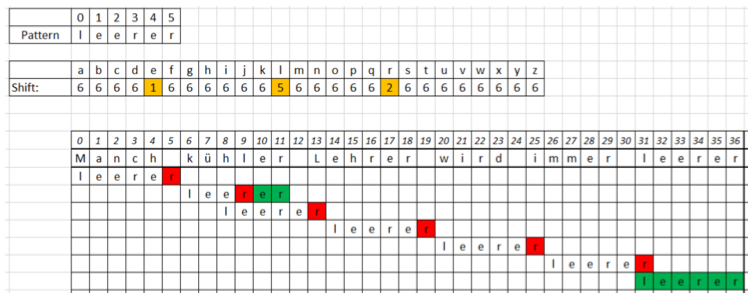
\includegraphics[width=\linewidth]{images/boyermoore}

\begin{minted}[breaklines]{java}
    public int firstMatch(String text, String pattern) {

        int[] shift = allShifts(pattern);

        int l = pattern.length(), i = 0, j = l - 1; // Warum?
        while (i + l <= text.length() && j >= 0) {

            j = l - 1; // Warum?

            while (j >= 0 && pattern.charAt(j) == text.charAt(i + j)) {
                  j--;
            }

            if (j >= 0) {
                i = i + shift[text.charAt(i + l - 1)];
            }
        }
        return (i + l <= text.length()) ? i : -1;
    }
\end{minted}
\input{inhalt/programmverifikation}
\section*{Rekursion}
\subsection*{DrawCricles}
\begin{minted}[breaklines]{java}
 private void drawCircles(Graphics g, int left, int top, int size) {
     if (size >= 8) {
         g.drawOval(left, top, size, size);
         int s = size / 2;
         drawCircles(g, left, top + s/2, s); //  links
         drawCircles(g, left + s, top + s/2, s); //  rechts
     }
}
\end{minted}

\subsection*{DrawSquares}

\begin{minted}[breaklines]{java}
private void drawSquares(Graphics g, int left, int top, int size) {
    left = left + margin;
    top = top + margin;
    size = size - 2 * margin;
    if (size >= 4) {
        g.drawRect(left, top, size, size);
        int s = size / 2;
        drawSquares(g, left, top, s); // oben links
        drawSquares(g, left + s, top, s); // oben rechts
        drawSquares(g, left + s, top + s, s); // unten rechts
    }
}
\end{minted}

\subsection*{DrawLines}
\begin{minted}[breaklines]{java}    
void drawFigure(Graphics g, int x, int y, int len, int level) {

    if (level >= 0) {
        len = len / 3;
        drawFigure(g, x, y, len, level - 1);
        drawFigure(g, x + len, y + len, len, level - 1);
        drawFigure(g, x + 2 * (len), y, len, level - 1);
    } else {
        g.drawLine(x, y, x + len, y);
    }
}
\end{minted}

\subsection*{DrawStars}
\begin{minted}[breaklines]{java}    
private void drawFigure(int lineSize, int level) {
   
    if(level > 0) {
    	drawFigure(lineSize/3, level - 1);
    	turnLeft(60);
    	drawFigure(lineSize/3, level - 1);
    	turnRight(120);
    	drawFigure(lineSize/3, level - 1);
    	turnLeft(60);
    	drawFigure(lineSize/3, level - 1);
    } else {
    	draw(lineSize/3);
    	turnLeft(60);
   		draw(lineSize/3);
   		turnRight(120);
   		draw(lineSize/3);
   		turnleft(60);
   		draw(lineSize/3);
   	}
}
\end{minted}


\subsection*{DrawTriangles}

\begin{minted}[breaklines]{java}    
private void drawRecTriangles(Point p1, Point p2, Point p3, int depth) {
  	if(depth > 0) {
  		drawTriangle(p1, p2, p3);
  		drawRecTriangles(p1, midPoint(p2, p3), midPoint(p3, p1), depth -1);
  		drawRecTriangles(midPoint(p1, p2), midPoint(p2, p3), p3, depth -1);
  		drawRecTriangles(midPoint(p1, p2), p2, midPoint(p3, p1), depth -1);
  	}
}
\end{minted}

\subsection*{Fibonacci}

\begin{minted}[breaklines]{java} 
public static long fiboRec(int n) {
    if (n > 1) {
        return fiboRec(n - 1) + fiboRec(n - 2);
    }
    return n;
}

public static long fiboIter(int n) {
    if (n < 1) return n;
    else {
        int i = 1;
        long f = 1, f1 = 0; 
        while (i < n) { // Invariante: f = f(i) AND f1 = f(i-1)
            f = f + f1;
            f1 = f - f1;
            i = i + 1;
        }
        return f;
    }
}
\end{minted}
\section*{Merge-Sort}

$T(n) = 2*T(n/2) + n$

\textbf{Worst-, Best- und Average-Case:} 

$\mathcal{O}(n*log(n))$, selten Worst-Case $\mathcal{O}(n^2)$

Zusätzlicher Speicher von $\mathcal{O}(n)$

\begin{minted}[breaklines]{java}
    private void sort(int[] a, int beg, int end) {

        if (end - beg > 1) {
            int m = (beg + end) >>> 1;
            sort(a, beg, m);
            sort(a, m, end);
            merge(a, beg, m, end);
        }
    }

    private void merge(int[] a, int beg, int m, int end) {
        int[] b = new int[end - beg];

        int i = 0, j = beg, k = m;
        while (j < m && k < end) {
            if (a[j] <= a[k]) b[i++] = a[j++];
            else b[i++] = a[k++];
        }
        while (j < m) {
            b[i++] = a[j++];
        }
        while (i > 0) {
            --i;
            a[beg + i] = b[i];
        }
    }

\end{minted}

\subsection*{Merge Inplace}

\begin{minted}[breaklines]{java}
    private void sort(int[] a, int beg, int m, int end) {

		int j = beg, k = m;
		while(j != k && k != end) {
			if(a[j] <= a[k]){
				j++;
			} else {
				int temp = a[k];
				for(int i = k; i > j; i--){
					a[i-1] = a[i];
				}
				a[j] = temp;
				k++;
				j++;
			}
		}
        
    }
\end{minted}

\subsection*{Merge Halber-Speicher}

\begin{minted}[breaklines]{java}
    private void merge(int[] a, int beg, int m, int end) {
		int[] b = new int[m-beg];
		for(int i = beg; i < m; i++) {b[i-beg] = a[i];}
		int i = beg, j = 0, k = m;
		while (0 < (m - beg) || k < end) {
			if(b[j] < a[k]){
				a[i] = b[j]; i++; j++;
			} else {
				a[i] = a[k]; i++; j++;
			}
			
		}
		while(j < (m-beg)){
			a[i] = b[j]; i++; j++;
		}
    }
\end{minted}
\section*{Quick-Sort}

$T(n) = 2*T(n/2) + a*n + b$

\textbf{Best-Case:} $\mathcal{O}(n*log(n))$

\textbf{Average-Case:} $\mathcal{O}(log(n))$

\textbf{Worst-Case:} $\mathcal{O}(n^2)$

Zusätzlicher Speicher von $\mathcal{O}(log(n))$

\begin{minted}[breaklines]{java}

	static void sort(int[] a, int beg, int end) {

        if (beg < end) {
            int x = a[(beg + end) / 2];
            int i = beg;
            int j = end;

            while (i <= j) {
                while (a[i] < x) i++;
                while (a[j] > x) j--;
                if (i <= j) {
                    int t = a[i];
                    a[i] = a[j];
                    a[j] = t;
                    i++;
                    j--;

                }
            }
            sort(a, beg, j);
            sort(a, i, end);
        }
    }

    private void sort(SortData a, int beg, int end) {

        if (beg < end) {
            int x = (beg + end) / 2;
            int i = beg, j = end;
            while (i <= j) {
                while (a.less(i, x)) i++;
                while (a.less(x, j)) j--;
                if (i <= j) {
                    a.swap(i, j);
                    if (i == x) {
                        x = j;
                    } else if (j == x) {
                        x = i;
                    }

                    ++i;
                    --j;
                }
            }
            sort(a, beg, j);
            sort(a, i, end);
        }
    }
    
    
   	void sort(int[]a, int beg, int end) {
        if(beg >= end) return;
        if(a[beg] > a[end]) swap(a, beg, end);
        int p1 = a[beg], p2 = a[end];

        int i = beg + 1, k = i, j=end;
        while(k != j ){
            if(a[k] <= p1){
                swap(a,i,k); i++; k++;
            }else if(a[k] <= p2){
                k++;
            }else{
                j--; swap(a,k,j);
            }
        }
        sort(a, beg, i-1);
        sort(a, i, j-1);
        sort(a, j, end);
    }

\end{minted}
\subsection*{Quicksort Cutoff}
\begin{minted}[breaklines]{java}
private void quicksort(SortData data, int l, int h) { 
	if (h - l > CUT_OFF) {
		int i = l, j = h, m = (l + h) / 2; 
		while (i <= j) {
			while (data.less(i, m)) i++; 
			while (data.less(m, j)) j--; 
			if (i <= j) {
				data.swap(i, j);
			if (i == m) m = j;
				else if (j == m) m = i; i++; j--;
			}
		} 
		quicksort(data, l, j);
		quicksort(data, i, h);
	} else
		insertionSort(data, l, h);
	}
}
private void insertionSort(SortData data, int beg, int end) {
	for (int i = beg + 1; i <= end; i++) {
		int j = i;
		while (j > beg && data.less(j, j - 1)) { data.swap(j, j - 1); j--; } }
}
	
\end{minted}
\
\section*{Summenformeln}

\textbf{Gauss}
\begin{equation}
    \sum_{k=1}^{n} k = \frac{n(n+1)}{2}
\end{equation}

\textbf{Gerade Zahlen}
\begin{equation}
    \sum_{k=1}^{n} 2k = n*(n+1)
\end{equation}

\textbf{Ungerade Zahlen}
\begin{equation}
    \sum_{k=1}^{n} 2*(k-1) = n^2
\end{equation}

\textbf{Quadrat Zahlen}
\begin{equation}
    \sum_{k=1}^{n} k^2 = \frac{n*(n+1)*(2n+1)}{6}
\end{equation}

\textbf{Kubische Zahlen}
\begin{equation}
    \sum_{k=1}^{n} k^3 = (\frac{n*(n+1))}{2})^2
\end{equation}

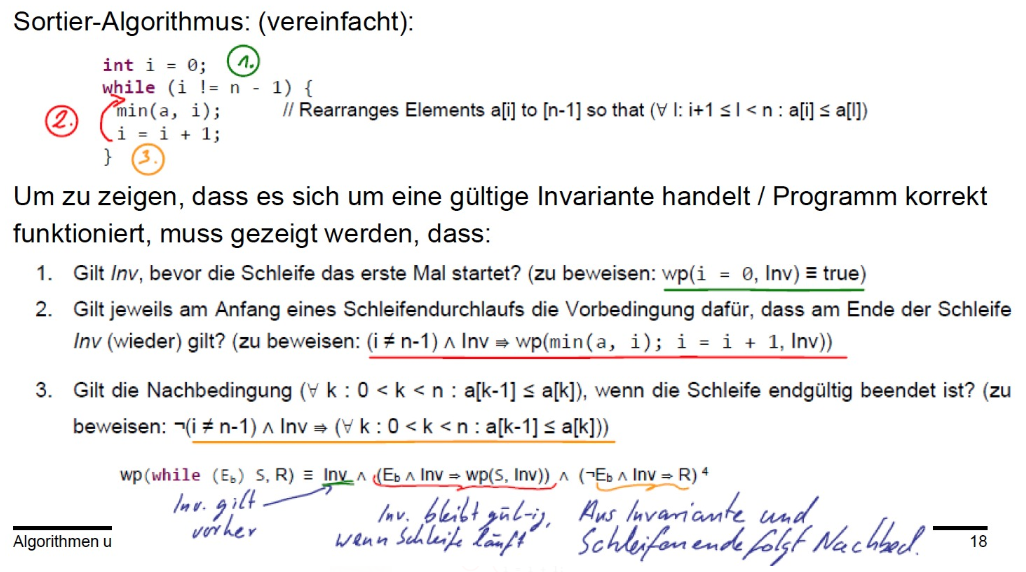
\includegraphics[width=\linewidth]{images/invariante}
\section*{Backtracking}
\subsection*{Backtracking}
\begin{minted}{java}
	private boolean solve(___data___, int row) {
        if (isSolved()) return true;
        else {

            // Optimierung

            loop(____) {
                set(____);
                if (!solve(___data___, row + 1))
                    unset(_____);
            }
            return false;
        }
    }
\end{minted}
\subsection*{Dame}
\begin{minted}[breaklines]{java}
    public boolean solve(boolean[][] board, int row) {
        if (row == board.length) return BoardChecker.isValid(board);

        int col = 0;
        boolean solved = false;

        while (col < board[row].length && !solved) {
            board[row][col] = true;

            solved = solve(board, row + 1);

            if (!solved)
                board[row][col] = false;
            col++;

        }
        return solved;
    }
\end{minted}
\subsection*{Springer}
\begin{minted}[breaklines]{java}
    public boolean move(int x, int y, int step) {
        visit(x, y, step);
        if (step == size * size) return true;

        List<Move> nextMoves = calcNextMoves(x, y);
        warnsdorffRule(nextMoves);

        for (Move move : nextMoves) {
            boolean solved = move(move.getX(), move.getY(), step + 1);
            if (solved) return true;

        }
        unvisit(x, y);
        return false;
    }
\end{minted}
\subsection*{Knappsack}
\begin{minted}[breaklines]{java}
    private static void pack(int i) {
        cnt++;
        if (i < weight.length) {
            pack(i + 1);
            packItem(i);
            pack(i + 1);
            unpackItem(i);
        } else if (totWeight <= capacity && totValue > maxValue) {
            maxValue = totValue;
        }

        if (sb.length() ==  8) System.out.println(sb);
        cnt--;
    }
\end{minted}
\subsection*{Bratkartoffel}
\begin{minted}[breaklines]{java}
private static void solve(int i) { if (i == weights.length) {
	if (minDifference > Math.abs(first - second)) 
		minDifference = Math.abs(first - second);
	} else {
		first = first + weights[i]; solve(i + 1);
		first = first - weights[i]; second = second + weights[i]; solve(i + 1);
		second = second - weights[i];
	}
}
\end{minted}
\subsection*{Sudoku}
\begin{minted}[breaklines]{java}
public boolean solve(int i, int j, int[][] cells) {
	if (i == 9) {
		i = 0;
		if (++j == 9) 
			return true; 
	}
	if (cells[i][j] != 0)  // skip filled cells
		return solve(i+1,j,cells);
	
	for (int val = 1; val <= 9; ++val) {
	    if (legal(i,j,val,cells)) {  
			cells[i][j] = val;       
			if (solve(i+1,j,cells))  
		    	return true;
	    	}
		}
	cells[i][j] = 0; // reset on backtrack
	return false;
}
\end{minted}
\subsection*{Rat in a maze}
\begin{minted}[breaklines]{java}
boolean solve(int maze[][], int x, int y, int sol[][]) {
      // if (x, y is goal) return true 
      if (x == N - 1 && y == N - 1) {
          sol[x][y] = 1;
          return true;
      }

      // Check if maze[x][y] is valid 
      if (isSafe(maze, x, y) == true) {
          // mark x, y as part of solution path 
          sol[x][y] = 1;

          /* Move forward in x direction */
          if (solve(maze, x + 1, y, sol))
              return true; 

          // If moving in x direction doesn't give solution then Move down in y direction 
          if (solve(maze, x, y + 1, sol))
              return true; 

          // If none of the above movements works then BACKTRACK: unmark x, y as part of solution path 
          sol[x][y] = 0;
          return false;
      }

      return false;
}
\end{minted}
\subsection*{TSP}
\begin{minted}[breaklines]{java}
static int tsp(int[][] graph, boolean[] v, int currPos, int n, int count, int cost, int ans) { 
  if (count == n && graph[currPos][0] > 0){ 
      ans = Math.min(ans, cost + graph[currPos][0]); 
      return ans; 
  } 
  for (int i = 0; i < n; i++) { 
      if (v[i] == false && graph[currPos][i] > 0) { 

          // Mark as visited 
          v[i] = true; 
          ans = tsp(graph, v, i, n, count + 1, cost + graph[currPos][i], ans); 
          // Mark ith node as unvisited 
          v[i] = false; 
      } 
  } 
  return ans; 
} 
\end{minted}
\section*{Datentypen}
\subsection*{Bite}
\subsubsection*{2er Potenzen}
\begin{center}

\resizebox{\columnwidth}{!}{%
\begin{tabular}{|c|c|c|c|c|c|c|c|c|c|c|}
\hline
2${}^{10}$ & 2${}^{9}$ & 2${}^{8}$ & 2${}^{7}$ & 2${}^{6}$ & 2${}^{5}$ & 2${}^{4}$ & 2${}^{3}$ & 2${}^{2}$ & 2${}^{1}$ & 2${}^{0}$ \\ \hline
1024 & 512 & 256 & 128 & 64 & 32 & 16 & 8 & 4 & 2 & 1 \\ 
\hline
\end{tabular}}
\end{center}

\begin{center}
\resizebox{\columnwidth}{!}{%
\begin{tabular}{|c|c|c|c|c|c|c|c|c|}
\hline
2${}^{0}$ & 2${}^{-1}$ & 2${}^{-2}$ & 2${}^{-3}$ & 2${}^{-4}$ & 2${}^{-5}$ & 2${}^{-6}$ & 2${}^{-7}$ & 2${}^{-8}$ \\ \hline
1 & 0.5 & 0.25 & 0.125 & 0.0625 & 0.03125 & 0.015625 & 0.0078125 & 0.00390625 \\ 
\hline
\end{tabular}}
\end{center}
\subsection*{Bitshift}
$>>$ Right Shift signed (mit 1en auffüllen)\\
$>>>$ Right Shift unsigned (mit 0en auffüllen)\\
$<<$ Left Shift unsigned (mit 0en auffüllen)
\subsection*{Float}
\begin{center}
\resizebox{\columnwidth}{!}{%
\begin{tabular}{|c|c|c|c|c|c|c|c|c|c|c|c|c|c|c|c|c|}
V & \multicolumn{8}{c|}{Exponent 8 Bit} & \multicolumn{8}{c|}{Mantisse} \\ \hline
1 & 1 & 0 & 0 & 0 & 0 & 1 & 0 & 1 & 0 & 0 & 1 & 0 & 0 & 1 & 0 & ... \\ \hline
\end{tabular}}
\end{center}

V = \textbf{-1}

Exponent = 128 + 4 + 1 = 133 => 133 - 127 (Bias) = \textbf{6}

1.0010010 => Komma um 6 Stellen nach Rechts verschieben
1001001.0 = \textbf{73}

\subsubsection*{Dezimalzahl nach Floating Point}

-23.5
\begin{itemize}
\item[1.] Dezimal zu Binär: 00010111.1
\item[2.] Normalisieren: 00010111.1 => 0001.011110...
\item[3.] Exponent: 4 + 127 (Bias) = 131 => 1000 0011
\end{itemize}

\section*{Zeichen}
\subsection*{Hex zu Binär}
\begin{center}

\begin{tabular}{ll|ll}
\textbf{Hex} & \textbf{Bin} & \textbf{Hex} & \textbf{Bin} \\ \hline
\multicolumn{1}{l|}{0} & 0000 & \multicolumn{1}{l|}{8} & 1000 \\
\multicolumn{1}{l|}{1} & 0001 & \multicolumn{1}{l|}{9} & 1001 \\
\multicolumn{1}{l|}{2} & 0010 & \multicolumn{1}{l|}{A} & 1010 \\
\multicolumn{1}{l|}{3} & 0011 & \multicolumn{1}{l|}{B} & 1011 \\
\multicolumn{1}{l|}{4} & 0100 & \multicolumn{1}{l|}{C} & 1100 \\
\multicolumn{1}{l|}{5} & 0101 & \multicolumn{1}{l|}{D} & 1101 \\
\multicolumn{1}{l|}{6} & 0110 & \multicolumn{1}{l|}{E} & 1110 \\
\multicolumn{1}{l|}{7} & 0111 & \multicolumn{1}{l|}{F} & 1111
\end{tabular}

\end{center}

\begin{center}
	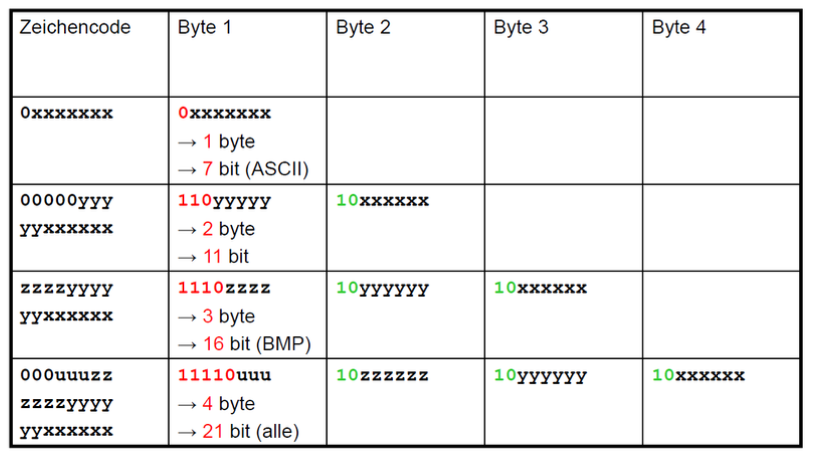
\includegraphics[width=10cm]{images/bitesneeded}
\end{center}

\section*{Suchen}
\subsection*{Sequenzielle Suche}
\begin{minted}{java}
int search(int[] arr, int x) {
    for(int i = 0; i < arr.length; i++) 
        if(arr[i] == x) 
            return i; 
    return -1; 
}
\end{minted}

\subsection*{Sequenzielle Suche mit Wächter}
\begin{minted}{java}
boolean search(int[] data, int value){
    int last = arr[n - 1];  
    arr[n - 1] = x;  
    int i = 0;  
    while (arr[i] != x)  
        i++;  
    arr[n - 1] = last;
    return (i < n - 1) || (x == arr[n - 1]);
}
\end{minted}

\subsection*{Binäre Suche}
\begin{minted}{java}
    int binSearch(int[] data, int value) {
        int l = -1, h = data.length;
        while (l + 1 != h) {
            int m = (l + h) >>> 1;
            if (data[m] < value) l = m;
            else h = m;
        }
        return h;
    }
\end{minted}
\subsection*{Max Sub Array}
\begin{minted}{java}
int maxSub(int[] data) {
  int max = 0, cur = 0;
  for (int end = 0; end < data.length; end++) {
    cur = cur > 0 ? cur + data[end] : data[end];
	if (cur > max) max = cur;
  }
  return max;
}
\end{minted}


\section*{Asymptotische Komplexität}
\subsection*{Komplexitätsklassen}
\begin{center}
	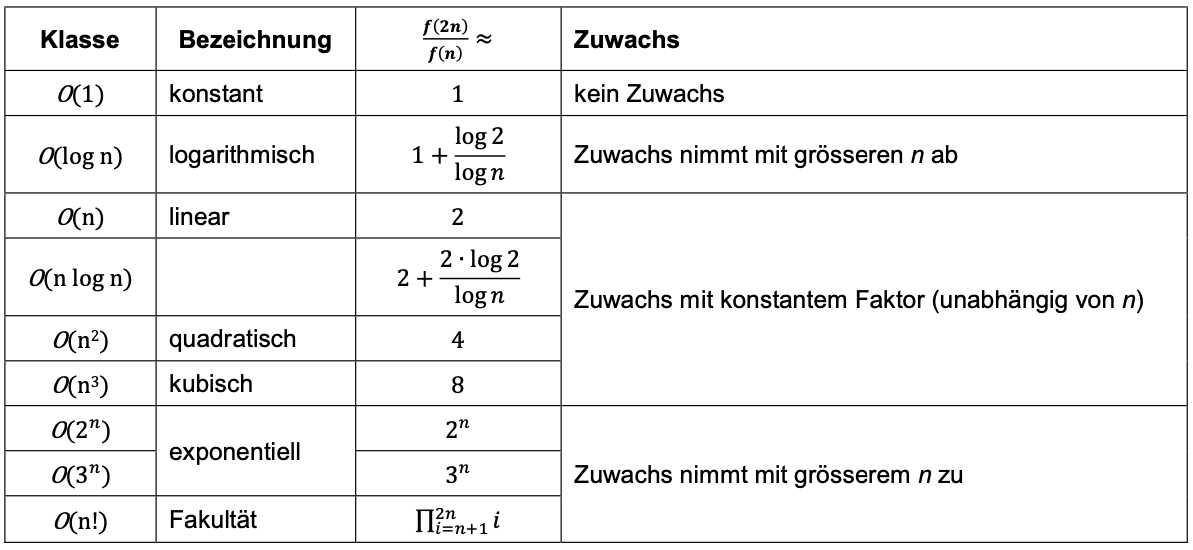
\includegraphics[width=10cm]{images/asympklassen}
\end{center}

$O(\log{}n)$ < $O(\sqrt{n})$ < $O(n)$

Binäre Suche: $O(\log{}n)$ % regular O

Sequenzielle Suche: $O(n)$ % regular O

\end{multicols*}
\end{document}